% !TeX encoding = UTF-8
\chapter{Grafische Benutzeroberfläche (GUI)}
\thispagestyle{fancy}
\label{Grafische Benutzeroberfläche}
In diesem Abschnitt erfolgt Beschreibung der Benutzeroberfläche der „Presentao-Applikation“ auf einem „Android-Device“. Diese GUI ist theoretisch nach dem kompilieren mit eventuell erforderlichen kleinen Anpassung auch für andere Plattformen/Geräten ähnlich abgebildet und verwendbar. Erfolgreich getestet ist die App allerdings derzeit nur für Android (4.3 + 4.4) und Windows.
\section{Bedienkonzept}
Das, aus den Anforderungen abgeleitete, Bedienkonzept bietet die Grundlage der strukturellen Gestaltung dieser App.
\subsection{Benutzerführung}
Die implementierte Benutzerführung stellt den intuitiven, effizienten und sinngemäßen Gebrauch der App sicher. In den Abbildungen XXX-XXX ist der Ablauf dargestellt.
\subsubsection{Start der App}
Benutzer der App erhalten zu nach dem Programmstart lediglich die Möglichkeit auf "Los!" die geführten Anfangseinstellungen zu beginnen.
\subsubsection{Auswählen der eigenen Rolle}
Die Auswahl der Rolle des Benutzer ist für den weiteren Aufbau der GUI entscheidend weshalb diese sich nicht überspringen lässt.
Zu dieser wichtigen Entscheidung kann der Benutzer jederzeit zurück navigieren.
\subsubsection{Netzwerkeinstellungen als Sprecher oder Zuhörer}
Wie in den Abbildungen XXX-XXX zu erkennen, ist ein grüner Pfeil erschienen um zu der Rollenauswahl zurück zu navigieren. Die notwendigen Einstellungen unterscheiden sich wesentlich je nach Rolle, und sind ebenfalls nicht überspringbar. Gemeinsame ist, für den Verbindungsaufbau zum Server, die Eingabe der IP-Addresse. ... 
\subsubsection{Kontextwechsel beim Sprecher oder Zuhörer}
Durch Bestätigen der Einstellungen auf "Übernehmen" wechselt die Ansicht automatisch zur "Pdf-Ansicht" und der grüne Pfeil verschwindet. Jetzt lässt sich durch ein Menü-Icon, dass dessen Platz eingenommen hat (siehe Abbildung XXX), eine Liste mit Navigationsmöglichkeiten öffnen. Die Liste beinhaltet neben Rollenauswahl, Netzwerkeinstellungen und der Pdf-Ansicht, für den Sprecher zusätzlich STEUERUNGSEINSTELLUNGEN.
\subsection{Pdf-Ansicht}
Sprecher und Zuhörer haben wie in Abbildung XXX dargestellt einen unterschiedlichen Aufbau. Als Zuhörer hat man einen Synchronisations-Icon. Dem Sprecher kann in einer Toolbar über Icons Steuerungselemente schnell aktivieren oder deaktivieren.
\subsubsection{Synchronisation}
Alle 5 Sekunden wird gefragt ob.... Oder nur bei betätigen oder Seitenwächsel des Sprechers.
\subsubsection{Toolbar-Icons}
Von Links nach Rechts: Audioerkennung, Bilderkennung, Beschleunigungserkennung
\paragraph{Ein Paragraph}$\;$\\
E
\subsection{Erweiterte Bedienmöglichkeiten}
Diese Applikation zeichnet sich besonders durch die erweiterten Bedienmöglichkeiten aus. Neben dem Aktivieren der Steuerungsoptionen in der Pdf-Ansicht über die Toolbar, kann man diese Optionen beim Sprecher über das Listenmenü in eigenen Seiten mit Hilfetext öffnen und anpassen.
\section{Softwarekonzept}
Das Softwarekonzept dient der Umsetzung des Bedienkonzepts mit "Qt-Creator" programmiert in C++ und Qml. Der Qt-Creator ist dafür wegen der Plattformunabhängigkeit ausgewählt.
\subsection{Zustandssteuerung}
Die Realisierung der Grafische Oberflächen entsprechend bisheriger Einstellungen ist über Zustände einer Variablen "appState" realisiert, die sich die aktuellen Einstellungen bzw. den Ort merkt und entsprechend Informationen mittels der Objekteigenschaft "visible" ein oder ausblendet.
\subsubsection{Zustände}
E
\paragraph{Ein Paragraph}$\;$\\
E

\begin{figure}[ht!]
	\centering
	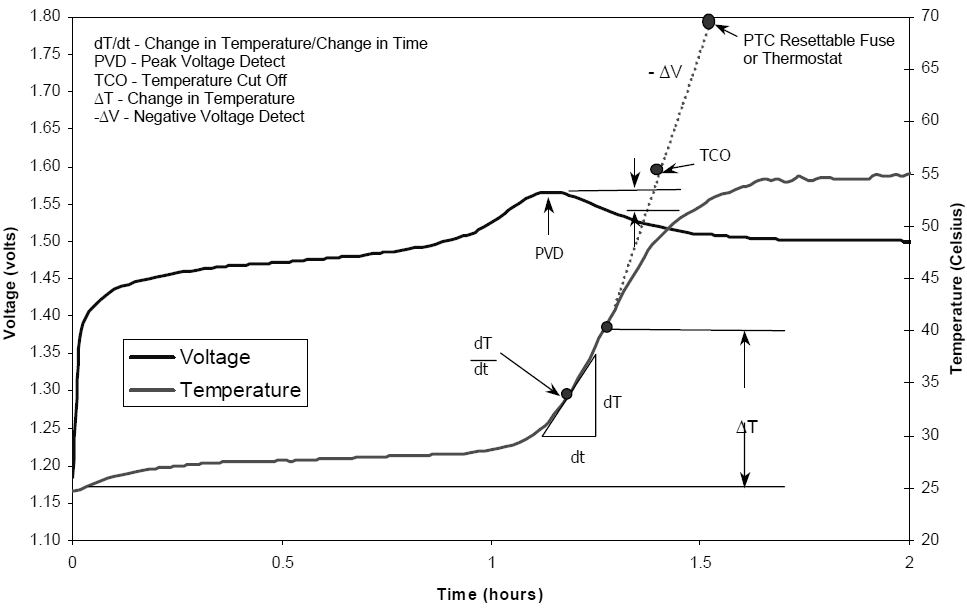
\includegraphics[angle=0,width=14cm]{LatexBeispiel/Bilder/Ladeschlussbw.png}
	\caption{Ladeschlusserkennungen, Harding Battery Handbook\cite{Harding}}
	\label{Ladeschluss}
\end{figure}

\newpage
So kann Code eingefügt werden.
\begin{lstlisting}[frame=single,breaklines=true,basicstyle=\tiny,language=C,label={PWMStart},caption={Kommentierter Start der PWM}]
/*! \brief Starts the PWM
* 
* To make sure that the PWM behaves correctly after a Compare Bit Change the PWM is started and reset with a software trigger.
*/
static void vStartPwm( void )
{
tc_start( &AVR32_TC0, PWM_CHANNEL );
tc_software_trigger( &AVR32_TC0, PWM_CHANNEL );
}
\end{lstlisting}

\subsection{Verbindungsaufbau}
Die Realisierung der 
\section{Ausblick}
Wir haben uns einige zusätzliche Funktionalitäten überlegt, die den Wert der Applikation für Zuhörer und Sprecher steigern könnte.\\
Erweiterungen für den Sprecher:\\
- Blättern in einer Pdf ohne dass ein Update auf dem Server erfolgt\\
Erweiterungen für den Zuhörer:\\
- Einstellen der Zeit die vergehen soll bis sich die Applikation synchronisiert\\